\chapter{Proof Extraction}
\label{chapter:chapter_3}

\chapabstract{\textit{What good is a program that only lives on paper?}}

With our theorycrafting over, we have in our hands an uninstantiated descriptive model of syntactic and semantic composition, promising to capture dependency relations while keeping both its feet set firmly in type theory.
Unfortunately, it is well attested by now that ``all models are wrong...''~\cite{doi:10.1080/01621459.1976.10480949}.
Any promise of theoretical universality, cognitive plausibility, linguistic intrinsicness or what have you, would require some degree of handwaving and conjencturing that I am not comfortable with.
What is undisputable, however, is the nobility of our goals and the purity of our tools: the \textit{omniversality} of the $\lambda$ calculus~\cite{wadler2015propositions} asserts that our modeling approach is not some ad hoc machinery designed to tackle a highly localized problem, but the one and only programming language ever worth writing. 
Beyond purpose and methodology, and having \textit{a priori} given up any ideation of truth, the only measure of success for our model is that of its utility (``...but some are useful'', ~\cite{doi:10.1080/01621459.1976.10480949}).
This sets up a new research imperative: we must prove the model useful!

``Oof, that's a tricky one'', you might say, and you wouldn't be wrong.
Thankfully, there are two tried and tested ways to proceed.
The first is the way of the scholar, which requires a rare combination of high intellectual capacity, strong persuasive skills and a pinch of luck.
It starts off with some profound abstract thinking, gradually overtaken by agressive campaigning: bashing the competition at workshops and conferences, making bold claims and generating traction at any chance given (optionally over social media platforms, for the modernists), eventually building a cult of personality, and finally resting on your laurels as the hype becomes self-sustainining; at long last, utility affirmed by popular approval.
This path, sometimes called the scientific method, is a rather involved and painstakingly slow process, a high stakes gamble that only starts yielding profits in the long run; as such, it greatly benefits from the nourishment of a stable work environment.
More befitting the modern paradigm of the mobile, adaptive, multi-purpose researcher is the alternative path, the way of the engineer.
A shorter term investment, it requires only the acquirable skills of endurance and hardheadedness, and offers a recipe that's easier to follow: simply swing at it until it cracks.
After a lot of obsessive iteration and self-correction (interchanged with the occasional feeling of despair), (f)utility will sooner or later be affirmed by cold, hard numbers.
We'll go for this one.

This choice has some methodological repercussions.
Under more tranquil circumstances, we'd wait for the theory to be disseminated, criticized, adapted, error-corrected and returned to sender, before finally moving on; it being a theory of language, this would entail a thorough qualitative analysis of several kinds of linguistic phenomena, coupled with a theoretical investigation of what it can or cannot adequately capture.
We are however in a compressed timeframe, forcing our hand into putting it straight to the test; the pragmatic approach is then to try and directly align it with real-world linguistic data at scale, and hope for the best.
The process, called \textit{proof extraction}, revolves around ``proving''  some source corpus of syntactically annotated sentences via the design and application of an algorithm tasked with translating the existing annotation format into derivations of the target grammar -- in our case, a grammar of dependency-enhanced compositional assembly.
Proof extraction serves a ternary purpose.
One, it gives us access to an uncompromisingly realistic testbed upon which we can immediately inspect and iteratively finetune the specifics of the grammar logic.
Two, it fills in for a strict and impartial external critic in providing a quantitative evaluation regime -- at each point in time, we are able to measure the proportion of source analyses (and corresponding linguistic phenomena) the algorithm provides a (reasonable) output for.
And three, the end-yield of this process has merit of its own.
As a derived dataset, it is first a building block necessary for populating the computational toolshed of the theory, and also a public resource for the world to with as they please.

\section{Preliminaries}
\subsection{The Dutch Language}
For our linguistic inquiries, the focus will be on Dutch.
Other than being the language I was contractually obliged to conduct this research on, Dutch is an interesting specimen, the idiosyncracies of which have in the past proven quite a topic of debate for others, and a source of headaches for myself.
I don't have any intention (or delusion of competence) to casually throw a detailed exposition of the Dutch grammar here, but a brief and superficial typological overview might help smooth the transition into the what is to come.
If the section has the opposite effect to the one intended, know that I'll hold no grudge if you skip ahead.

But first things first.
Dutch is a West Germanic language, spoken primarily in the Low Countries within Europe by some 25 million speakers.
Owing to the Netherlands' nasty colonial history, Dutch has left a noticeable mark on the global linguistic atlas: it has played a primary role in the evolution of Afrikaans and, to a far lesser extent, Indonesian, while native Dutch speakers can be found as far as South America and the Dutch Carribean region.
Demographics aside, the language is said to be one of the closest relatives of English and German, sharing many of their morphosyntactic characteristics -- we'll go through some of those together.
The abbrevations in the glosses to follow are industry standard, you can find their transcriptions in Table~\ref{table:gloss_abbreviations} of Appendix~\ref{sec:abbrevations}.
Any internal inconsistencies are deliberate: I am trying to gloss only those features relevant to the local discussion.

\subsubsection{The Noun Phrase}
\paragraph{Nouns}
Dutch nouns have three grammatical genders: the masculine, the feminine and the neuter.
The masculine and feminine genders are morphologically indistinguishable -- telling them apart is done on the basis of the lexicon alone.
\begin{exe}
\ex\label{gloss:genders}
\begin{xlist}
\ex
\gll \textit{de} \textit{aard}\\
the earth(\abbrv{m})\\
\ex
\gll \textit{de} \textit{zee}\\
the sea(\abbrv{f})\\
\ex
\gll \textit{het} \textit{bos}\\
the forest(\abbrv{n})\\
\end{xlist}
\end{exe}
There's two numbers, the singular and the plural, the latter constructed with the aid of the suffix \textex{-en} or rarely \textex{-s}, depending on the noun.
\begin{exe}
\ex 
\begin{xlist}
\ex
\gll \textit{de} \textit{zeven} \textit{zee-\"{e}n}\\
the seven sea-\abbrv{pl}\\
\glt{`the seven seas'}
\ex
\gll \textit{de} \textit{trekvogel-s}\\
the  migratory.bird-\abbrv{pl}\\
\glt{`the migratory birds'}
\end{xlist}
\end{exe}
Case markings are not overtly realized, except for some mostly frozen leftovers from the distant past -- their functionality has largely been replaced by word order constraints, with the indirect object (formerly in the dative) preceding the direct object (formerly in the accusative), and periphrastic constructions, with the preposition \texttr{aan}{to} used to indicate indirect objects (see Gloss~\ref{gloss:ido} later on), and \texttr{van}{of} to substitute the genitive.
\begin{exe}
\ex
\gll \textit{het} \textit{oog} \textit{van} \textit{de} \textit{geest}\\
the eye of the mind\\
\glt{`the mind's eye'}
\end{exe}
A cute peculiarity of Dutch is the strikingly common use of a productive diminutive form, denoting either small size or an affectionate disposition -- diminutives are formed with the suffix \textex{-tje} or regionally \textex{-ke}, and are always neuter (notice the gender change of Gloss~\ref{gloss:gender_change}).

\paragraph{Determiners}
Determiners precede the noun and match its gender and number.
There are two articles: the definite, and the indefinite.
The definite has two singular forms \textex{de}/\textex{het} (non-neuter/neuter) and a single plural \textex{de}. 
Non-neuter forms are used for both masculine and feminine (refer back to Gloss~\ref{gloss:genders}).
\begin{exe}
\ex\label{gloss:gender_change}
\begin{xlist}
\ex
\gll de klein-e vogel\\
the(\abbrv{nn.sg}) small-\abbrv{def} bird\\
\glt{`the small bird'}
\ex
\gll het klein-e vogel-tje\\
the(\abbrv{n.sg}) small-\abbrv{def} bird-\abbrv{dim}\\
\glt{`the small birdie'}
\end{xlist}
\end{exe}
The indefinite \textex{een} is gender-agnostic, and has no plural form.
\begin{exe}
\ex
\begin{xlist}
\ex\label{gloss:indef_adj_sg_n}
\gll een donker lied\\
a dark song\\
\glt{`a dark song'}
\ex 
\gll donker-e lied-eren\\
dark-\abbrv{pl} song-\abbrv{pl}\\
\glt{`dark songs'}
\end{xlist}
\end{exe}
Indefinite pronouns can be used to convey universal or existential quantification and negation, materializing as substitutes for determiners (e.g. \texttr{alles}{all}, \texttr{sommige}{some}, \texttr{geen}{no}, etc.), or as stand-alones (e.g. \texttr{iets}{something}, \texttr{niets}{nothing}, etc.).
\begin{exe}
\ex
\gll Alle mensen willen iets, sommige willen alles.\\
all people want something some want everything\\
\glt{`All people want something, some want everything.'}
\end{exe}
Possessive and demonstrative pronouns can also enact determiners, both uninflected (except for the first person plural \textex{ons} which inflects like an indefinite adjective, see next paragraph).
\begin{exe}
\ex
\gll De eend is mijn favoriet vogel.\\
the duck is my favorite bird\\
\glt{`The duck is my favorite bird.'}
\ex\label{gloss:ido}
\gll Het bos is onz-e tempel.\\
the forest is our-\abbrv{def} temple\\
\glt{`The forest is our temple.'}
\end{exe}
Demonstrative pronouns come in two major flavours: the proximal \textex{deze/dit} (plural \textex{deze}) and the distal \textex{die/dat} (plural \textex{die}).
The last two do double duty as relative pronouns -- more on that later.
When used to substitute (rather than determine) a noun in a copula, each variant reverts to its neuter singular form.
\begin{exe}
\ex
\begin{xlist}
\ex
\gll Deze bergen zijn hoog.\\
these(\abbrv{pl}) mountains are tall\\
\glt{`These mountains are tall.'}
\ex
\gll Dit zijn mijn bergen.\\
this(\abbrv{n}) are my mountains\\
\glt{'These are my mountains.'}
\end{xlist}
\end{exe}

\paragraph{Adjectives}
Adjectives used as nominal modifiers find their place between the determiner and the head noun.
They appear inflected with an \textex{-e} affix in all cases except for the idefinite use with a neuter singular noun (refer back to Gloss~\ref{gloss:indef_adj_sg_n}, contrast with \ref{gloss:gender_change}).
The same affix applies to nominalized adjectives, which can allow the ommission of a contextually implied noun, or be used independently as an abstract concept or a quantifying property.
\begin{exe}
\ex
\gll dood aan het heilig-e\\
death to the holy-\abbrv{nmlz}\\
\glt{`death to the holy'}
\ex
\gll De zachtmoedig-en zullen niets be\"{e}rven.\\
the meek-\abbrv{nmlz.pl} shall nothing inherit(\abbrv{inf})\\
\glt{`The meek shall inherit nothing.'}
\end{exe}
An alternative inflection with a \textex{-s} affix marks the partitive use, when the adjective modifies an indefinite pronoun.
\begin{exe}
\ex
\gll iets ernstigs-s\\
something grave-\abbrv{ptv}\\
\glt{`something grave'}
\end{exe}
The language provides acccess to a comparative and a superlative form, via the affixes \textex{-er} and \textex{-ste} respectively, or periphrastically with \texttr{meer}{more} and \texttr{meest}{most}.
\begin{exe}
\ex
\gll \textit{het} \textit{donker-ste} \textit{lied}\\
the(\abbrv{n.sg}) dark-\abbrv{sup} song\\
\glt{`the darkest song'}
\end{exe}

\paragraph{Personal Pronouns}
Noun phrases can be substituted by personal pronouns, which in Dutch are morphologically marked for case and gender.
The nominative is used for the subject position, the genitive corresponds to the possessive determiners discussed earlier, and the accussative is used to denote objects.
\begin{exe}
\ex
\gll Ik zie een vreemde man in de spiegel.\\
I(\abbrv{nom}) see a strange man in the mirror\\
\glt{`I see a strange man in the mirror.'}
\ex
\gll Hij merkt mij op.\\
he(\abbrv{nom}) perceives me(\abbrv{acc}) on\\
\glt{`He notices me.'}
\end{exe}
A dative form is sometimes exceptionally used for indirect objects in the third person plural.
Depending on the regional variation, personal pronouns must match the grammatical gender of the noun they refer to, or simply default to the neuter (reserving the masculine and feminine forms for animates).
Third person singulars are also interchangeable with the appropriate demonstratives.
Personal pronouns come in two variants: the stressed (emphatic) and the unstressed (standard).

\subsubsection{The Verb}
\paragraph{Conjugation}
In their citation form, verbs match their infinitival versions, regularly consisting of the verbal stem plus \textex{-en}.
Verbal conjugation patterns distinguish between two grammatical tenses, the non-past and the past, and three moods, the indicative, the subjunctive and the imperative, of which the first two are morpohologically conflated.
Each pattern is parameterized by person and number.
Aspectual flavours, passivization and an explicit future are accessible as productive constructions with modals, the latter being the common culprits of irregular conjugation.

\paragraph{Participles}
Participles exist for both tenses, and have a multitude of uses.
The present participle is formed by affixing \textex{-de}, and is commonly employed as an duration-denoting adjective or adverb, always inflected in the first case, and optionally in the second.
\begin{exe}
\ex
\gll de zweven-de vrouw\\
the levitate-\abbrv{prs.ptcp} woman\\
\glt{`the levitating woman'}
\end{exe}
Rarely, it can be used as a complement to the auxiliary \texttr{zijn}{to be} to produce a kind of present continuous.
Present participles of transitives can attach to the end of their object nouns, appearing as fused compounds.
The past participle is more versatile.
Regular past participles are formed by prefixing \textex{ge-} to the verbal stem (morphophonological terms and conditions may apply) and substituting the infinitival suffix for either \textex{-t}, \textex{-d} or nothing, depending on the stem's last phoneme.
Like the present participle, it can be used as an adjective, denoting now a completed event.
\begin{exe}
\ex
\gll beelden met ge-sloten ogen\\
images with \abbrv{pst.ptcp}-close eyes\\
\glt{`closed eye visuals'}
\end{exe}
Combined with with the modal \texttr{hebben}{to have} (or exceptionally \textex{zijn} for unaccusatives and verbs of movement), it produces the perfect tense.
\begin{exe}
\ex
\end{exe}
Combined with the modals \texttr{worden}{to become} and \texttr{zijn}{to be}, it produces the passive voice and its perfect tense.

\paragraph{Infinitives}
Infinitival forms commonly occur as the verbal complements of a modal, auxiliary or perception verb.
\begin{exe}
\ex
\gll Ik wil slapen.\\
I want sleep(\abbrv{inf})\\
\glt{`I want to sleep.'}
\end{exe}
Depending on the modal, the preposition \texttr{te}{to}, or the discontinuous \texttr{om ... te}{to}, may be either necessary, optionally admissible or completely disallowed -- if one does manifest, it precedes the infinitive.
\begin{exe}
\ex
\gll Ik probeer te schrijven.\\
I try to write(\abbrv{inf})\\
\glt{`I try to write.'}
\end{exe}
The discontinuous variant is only selected for by specific verbs -- it can enclose linguistic material, like the infinitive's object or any adverbs modifying it.
\begin{exe}
\ex
\gll Ik dwing mezelf om wat te schrijven.\\
I force myself \_ something to write(\abbrv{inf})\\
\glt{`I force myself to write something.'}
\end{exe}
An infinitive directly following \textex{aan het} can combine with \textex{zijn} to construct the continuous aspect, in either the present or the past tense.
\begin{exe}
\ex
\gll Ik ben aan het schrijven.\\
I am in the write(\abbrv{inf})\\
\glt{`I am writing.'}
\end{exe}
Infinitives are also often nominalized, the resulting nominals being singular neuters.
\begin{exe}
\ex
\gll Het schrijven is pijnlijk.\\
The write(\abbrv{inf}) is painful\\
\glt{`The writing is painful.'}
\end{exe}

\paragraph{Separable Verbs} 
The verbal lexicon contains several compound items comprised of a preposition and a verbal stem, usually with a compositional meaning.
The stem is separated from its prepositional prefix when the verb heads a matrix clause, in which case the preposition is moved to the end of the clause -- in all other cases, including the finite form in subordinate clauses, the two remain attached.
When inflecting for the perfect, the prefix applies to the stem (i.e. after the preposition).

\subsubsection{The Sentence}
By far the most fun aspect of Dutch is its absolutely wild sentential word order.

\paragraph{Main Clauses}
The main clauses inspected so far emanate a false sense of safety, coming off as SVO at first glance, with participles used for the passive voice and the perfect tense pushed to the right edge of the clause.
The truth is far more sinister -- the verb is placed there only by exception, abiding by the V2 rule that has it appear second for matrix clauses only.
The effect becomes apparent when employing a preverbal adverb -- in Gloss~\ref{gloss:simple_smain_v2}, both the subject and its predicate complement follow the verb in a VSO pattern.


\paragraph{Questions and Imperatives}
When it comes to questions, things look familiar again.
Line in English, wh-questions begin with an interrogative pronoun or adverb (e.g. \texttr{wie}{who}, \texttr{wat}{what}, \texttr{welk}{which}, \texttr{waarom}{why} etc.), which is immediately followed by the conjugated verb (Gloss~\ref{gloss:simple_whq}).
In direct questions without an interrogative, as well as positive imperatives, the verb is placed first (Glosses~\ref{gloss:simple_sv1_q} and \ref{gloss:simple_sv1_imp}).
In negative imperative sentences and impersonal commands, the infinitival is placed last.

\begin{exe}
\ex
\begin{xlist}
\ex\label{gloss:simple_smain}
\gll Frans verkoop-t kaas.\\
Frans sell-\abbrv{prs.3sg} cheese\\
\glt{`Frans sells cheese.'}
\ex\label{gloss:simple_smain_v2}
\gll Morgen verkoop-t Frans kaas.\\
tomorrow sell-\abbrv{prs.3sg} Frans cheese\\
\glt{`Frans will sell cheese tomorrow.'}
\ex\label{gloss:simple_sv1_q}
\gll Verkoop-t Frans kaas?\\
sell-\abbrv{prs.3sg} Frans cheese\\
\glt{`Does Frans sell cheese?'}
\ex\label{gloss:simple_whq}
\gll Wie verkoop-t kaas?\\
who sell-\abbrv{prs.3sg} cheese\\
\glt{`Who sells cheese?'}
\ex\label{gloss:simple_sv1_imp}
\gll Verkoop kaas!\\
sell(\abbrv{imp}) cheese\\
\glt{`Sell cheese!'}
\end{xlist}
\end{exe}

\paragraph{Subordinate Clauses}
Subordinate clauses is where things really get interesting.
Unaffected by the V2 rule, the word order turns out to be SOV; this affects indirect questions, verbal complements and relative clauses alike.
Indirect questions are straightforward -- modulo the word order permutation, they match their direct counterparts.
\begin{exe}
\ex\label{gloss:embedded_q}
\gll Weet je wie kaas verkoopt?\\
know you who cheese sells\\
\glt{`Do you know who sells cheese?'}
\end{exe}
Infinitives in non-nested verbal complements are likewise just pushed to the end of their clause.
\begin{exe}
\ex\label{gloss:simple_vc}
\gll Frans wil koopman worden.\\
Frans wants merchant be(\abbrv{inf})\\
\glt{`Frans wants to be a merchant.'}
\end{exe}
Relative clauses are instigated by relative adverbs and pronouns.
Interestingly, the language does not make an overt distinction between an object- and a subject- relative pronoun; combined with the SOV word order, and the absence of case markings, the effect is that the two relative clause types end up having the exact same surface form when the grammatical gender of the antecedent noun and the non-gap embedded argument are the same -- contrast the two sentences below.
\begin{exe}
\ex\label{gloss:rc_ambiguity}
\begin{xlist}
\ex
\gll het geheim dat een bos verbergt\\
the secret(\abbrv{n}) that a forest(\abbrv{n}) hides\\
\glt{
\begin{enumerate}[topsep=0pt]
	\item `the secret the hides a forest'
	\item `the secret that a forest hides'
\end{enumerate}}
\ex
\gll de kerk die vuur opslokt\\
the church(\abbrv{nn}) that(\abbrv{nn}) vuur(\abbrv{n}) consumes\\
\glt{`the church that fire consumes'}
\end{xlist}
\end{exe}

The SOV order means that the chaining of verbs requiring non-finite complements inadvertently leads to \textit{verb clusters}, i.e. collections of two or more verbs situated within the dependent clause and adjacent to one another.
Verb clusters are marked by their inability to accommodate non-verbal material, and may follow a number of different word orders, which don't necessarily abide by the order of selectional dominance.
The question of which factors influence the grammaticality of word order variations  is a hot potato and a topic of active research for decades -- to make matters worse, these factors tend to differ between regional variations of the language.%
	\footnote{As a fun trivia,  out of the 6 possible orderings of 3-verb clusters, 4 to 5 were found admissible by Dutch speakers depending on the construction~\cite{3vc}.}
What follows are some simplified common observations -- the interested reader should find the thesis of~\citet{augustinus2015complement} a good entry point towards more detailed discussions.

For starters, bare infinitives usually follow their governor -- but: this is not necessarily the case for clusters of 2 verbs where the finite verb is a modal.
The first two  below depict the canonical and ``inverted'' word orders; the third example is ungrammaticaul due to the adjective \textex{naamloos} interrupting the cluster.
\begin{exe}
\ex\label{gloss:rusten_zal}
\begin{xlist}
\ex
\gll ... waar ik naamloos zal rusten\\
.... where I nameless will rest(\abbrv{inf})\\
\ex
\gll ... waar ik naamloos rusten zal\\
... where I nameless rest(\abbrv{inf}) will\\
\glt{`... where I will rest nameless'}
\ex[*]{\textit{... waar ik zal naamloos rusten}}
\end{xlist}
\end{exe}
Past participles used in the formation of the perfect or passive may occur either to the left or the right of the tense auxiliaries \textex{hebben} and \textex{zijn}, leading to either a German- or English- like construction.
\begin{exe}
\ex\label{gloss:green_vs_red}
\begin{xlist}
\ex
\gll ... omdat ik de eend ge-zien heb\\
... because I the duck \abbrv{pst.ptcp}-see have\\
\ex
\gll ... omdat ik de eend heb ge-zien\\
... because I the duck have \abbrv{pst.ptcp}-see\\
\glt{`... because I have seen the duck'}
\end{xlist}
\end{exe}
This gets complicated by the so-called IPP (\textit{Infinitivus Pro Participio}) effect, where a participle that selects for an infinitive changes to an infinitive itself, creating a cluster in the process -- once more, whether this substitution is mandatory, optional or altogether impossible is lexically decided.
\begin{exe}
\ex\label{gloss:ipp}
\begin{xlist}
\ex 
\gll Ik heb de eend ge-zien.\\
I have the duck \abbrv{pst.ptcp}-see\\
\glt{`I have seen the duck.'}
\ex
\gll Ik heb de eend zien vliegen.\\
I have the duck see(\abbrv{inf}) fly(\abbrv{inf})\\
\glt{`I have seen the duck fly.'}
\ex\label{gloss:ipp_tv}
\gll Ik heb de eend een nest zien maken.\\
I have the duck a nest see(\abbrv{inf}) make(\abbrv{inf})\\
\glt{`I have seen the duck make a nest.'}
\end{xlist}
\end{exe}
Next, the infinitival head of a dependent clause may be forced to occur directly after the verb dominating it, if the latter belongs to a closed set of so-called \textit{raising} verbs (i.e. the raiser is infixed between the infinitive to the right, and the infinitive's non-verbal arguments to the left).
These include modals like \texttr{willen}{to want} and \texttr{moeten}{must}, perception verbs like \texttr{horen}{to hear} and \texttr{zien}{to see}, and some nondescript verbs like \texttr{doen}{to do} and \texttr{laten}{to let}.
As before, they can be subcategorized as obligatory raisers and optional ones.
\begin{exe}
\ex
\gll Ik denk dat ik iemand hoor naderen\\
I think that I someone hear approach(\abbrv{inf})\\
\glt{`I think I hear someone approaching.'}
\end{exe}
Yet other verbs like \texttr{verplichten}{to forbid} select not a bare infinitive but a \textex{te}-marked infinitival phrase, which they leave intact at the end of the clause -- a phenomenon known as \textit{extraposition}.
The twist is that the intersection of extraposition verbs and raising verbs is non-empty -- \texttr{proberen}{to try}, for instance, can behave as either.

\goodbreak\begin{exe}
\ex\label{gloss:vr_vs_xpos}
\begin{xlist}
\ex
\gll \textit{Ik} \textit{denk} \textit{dat} \textit{hij} \textit{probeert} \textit{iets} \textit{te} \textit{zeggen}.\\
I think that he tries something to say(\abbrv{inf})\\
\ex
\gll \textit{Ik} \textit{denk} \textit{dat} \textit{hij} \textit{iets} \textit{probeert} \textit{te} \textit{zeggen}.\\
I think that he something tries to say(\abbrv{inf})\\
\glt{`I think that he is trying to say something'}
\end{xlist}
\end{exe}

Typology aside, Dutch verb clusters have been a favorite topic of debate for formal grammarians for a while now, since their construction requires expressive capacity beyond what a context-free grammar can offer, and thus brinking an end to any delusion that human languages are context-free~\cite[\textit{inter alia}]{huybregts1984weak,shieber1985evidence}.%
	\footnote{Or, depending on the reader, that Dutch is a human language.}%
The impenetrable nature of verb clusters means that verbs that partake in their construction may often be forced to detach from their arguments, or worse yet become stranded from them by the infixation of another verb in between -- in the dependency grammar paradigm, these discontinuities materialize as non-projective (or cross-serial) dependencies -- see Figure~\ref{figure:xdep_udparse} for an example.

\begin{figure}
	\centering
	\begin{tikzpicture}[t/.style={text height=1.5ex, text depth=.25ex, rectangle, outer sep=0pt}, node distance=10pt]
	\smaller
%%	\node[t] (1) 			
	\node[t] (1)			at (0, 0) {\w{ik}};
	\node[t] (2)			[right=10pt of 1] {\w{heb}};
	\node[t] (3)			[right=10pt of 2] {\w{de}};
	\node[t] (4)			[right=10pt of 3] {\w{eend}};	
	\node[t] (5)			[right=10pt of 4] {\w{een}};	
	\node[t] (6)			[right=10pt of 5] {\w{nest}};
	\node[t] (7)			[right=10pt of 6] {\w{zien}};
	\node[t] (8)			[right=10pt of 7] {\w{maken}};
	\draw[->] (2) [bend right=80] edge node [above] {\smaller[2]{nsubj}} (1);
	\draw[->] (2) [bend left=90] edge node [above] {\smaller[2]{vc}} (7);
	\draw[->] (2) [bend left=90] edge node [above] {\smaller[2]{obj}} (4);
	\draw[->] (4) [bend right=60] edge node [above] {\smaller[2]{det}} (3);
	\draw[->] (7) [bend left=70] edge node [above] {\smaller[2]{vc}} (8);
	\draw[->] (8) [bend right=90] edge node [above] {\smaller[2]{obj}} (6);
	\draw[->] (6) [bend right=60] edge node [above] {\smaller[2]{det}} (5);
	\end{tikzpicture}
	\caption{Crossing dependencies in the 2-verb cluster of Gloss~\ref{gloss:ipp_tv}.}
	\label{figure:xdep_udparse}
\end{figure}

\paragraph{Adverbs}
Last item on the agenda are adverbs, commonly enacted by uninflected adjectives.
When not appearing in the emphatic first position, adverbial phrases must occur after definite objects and before indefinite ones, their internal order following a time-manner-location pattern.
\begin{exe}
\ex
\gll Turkse varkens doden momenteel laf burgers in Koerdistan.\\
Turkish pigs kill currently coward(\abbrv{adv}) civilians in Kurdistan\\
\glt{`Turkish pigs are cowardly killing civilians in Kurdistan right now.'}
\end{exe}
Adverbial counterparts to pronouns make for locative adverbs (i.e. \textex{dit} becomes \texttr{hier}{here}, \textex{dat} becomes \texttr{daar}{there}, \textex{wat} becomes \texttr{waar}{where}, etc.). 
Unique among them is \textex{er} from the singular neuter personal pronoun \textex{het}, which finds use as an unstressed locative or a subject-filler for an impersonal passive.
\begin{exe}
\ex
\gll Er is geen zaken doen op een dode planeet.\\
there is no business make(\abbrv{inf}) on a dead planet\\
\glt{`There is no business on a dead planet.'}
\end{exe}
When a preposition would apply to a singular neuter pronoun, the adverbial form is commonly employed instead; their positions are inverted, and if they end up adjacent they become fused, giving rise to a so-called  pronominal adverb.
Pronominal adverbs are common in Dutch, and find use as interrogative adverbs or relative pronouns.
\begin{exe}
\ex
\begin{xlist}
\ex[*]{\textit{Wat prat je over?}}
\ex
\gll Waar praat je over?\\
what talk you about\\
\ex
\gll Waarover praat je?\\
what.about talk you\\
\glt{`What are you talking about?'}
\ex
\gll We praten erover.\\
we speak it.about\\
\glt{`We are talking about it.'}
\end{xlist}
\end{exe}


\subsection{Parsing vs. Parsing}
With this lengthy detour over, we arrive at some painful truths: if there's any message to take home, it's the sheer amount of complexity inherent in a natural language grammar.
Nominals come with a ton of morphosyntactic rules, exposing the fact that there's no syntactic entity as simple and unmarked as the idealized \np[s] we have extensively utilized in earlier chapters.
The erroneous ommission or addition of as much as an inflectional marking suffices to turn a phrase ungrammatical.
The same issue pesters verbal morphology -- combining a verb with its potential arguments requires solving a number of constraints relating to number and person (let aside any notions of semantic compatibility).
To see these constraints solved on the type level is not out of the question; it is in fact something modalities may prove useful in~\cite{moa} -- it is, however, a problem in its own right.
But these concerns are trivial compared to the monumental intricacies laid down by word order constraints.
For a language like Dutch, devising the type assignments and structural rules that exactly allow the word permutations admissible by the language is a tremendous undertaking that requires navigating a complex network of layered rules and exceptions subject to regional variety.

That is not to say that such endeavours are without merit; a formalism that presents itself as syntactic in nature yet fails to provide a general and transparent account of morphosyntactic and word order constraints wouldn't be particularly honest.
The above remarks bring forth, however, a question of priorities, and by implication put us at a juncture point.
We have on the one hand the option to pursue the Lambekian holy grail: the design of a substructural type system, the proof search over which should amount to a decision procedure capable of telling sentence and non-sentence apart.
Put in practical terms, we'd settle for nothing less than absolute alignment with the Dutch grammar; just enough expressivity to ensure no overgeneration, no undergeneration and a perfect resolution of any and all syntactic ambiguities.
The other option is perhaps more sober -- depending on our end-goals, we can check our ambitions to a more realistic level.
A focus on sentence formation, for instance, would justify some morphological concessions.
But since the focus here is on compositionality, we're given the chance for a much more radical leap: we can also skip word order altogether.

Now this might be met with some scepticism, but put down your pitchforks and let me explain.
In the type-logical setup, we'd follow the schema of Figure~\ref{figure:synsemtlg}: start from a strict syntactic logic, and then strip it down to its bare essentials to cast it into a logic of derivational semantics, the bare essentials in our case being linear implication and the dependency modalities.
With derivational semantics being itself the point of interest, why take the hard route instead of just going there directly?
This is somewhat akin to the abstract categorial grammar operationalization of Figure~\ref{figure:synsemacg}, which would have us start from a tectogrammatic logic, and transition to phenogrammar via a morphism (here left unimplemented).
A perhaps less stretched operationalization would involve a two-stage inferential setup, the first stage being the phase of logical meaning assembly, followed by a higher-level phase of structural reorganization and reordering (here we'll call it quits immediately after the first).
Put bluntly, this option allows us to sneak our way out of having to reason about the non-compositional aspects of syntax.%
	\footnote{An atonement to the ghost of Montague, returned to claim his dues.}
Obviously this alters the scope of our endeavours.
Before any regrettable accusations are thrown, consider that we need not be apologetic for the elephant in the room, namely overgeneration.
$\NLP_{\ddia, \bx}$ is \textit{not} intended to be the logic you put in generation mode, and its proof theory is \textit{not} Lambek's decision process.
Rather, its an adequately expressive formalism that can accommodate the duality of function-argument structures and dependency annotations we set out to capture.
The problem is more practical than theoretical: who is going to hand us these deep syntactic proofs if not for the morphism that was promised?
Suffice it to say this requires adopting a new notion of parsing (still well under the deductive paradigm): that of associating a well-formed input with the correct tectogrammatic analysis.
How exactly this is to be done doesn't need to concern us for now -- we'll cross that bridge when we get to it.

\subsection{Lassy}
To facilitate the agenda just established, what we need next is a sizeable resource of syntactic annotations that are both high-quality and sufficiently compatible to our needs.
Fortunately, the search is rather short -- the only candidate is also the perfect one: Lassy~\cite{van2013large}.

Lassy consists of two annotated corpora, containing sentences paired with a single analysis.
Analyses are provisioned by Alpino~\cite{van2006last}, a powerful parser that stands the test of time by combining a high quality handcrafted lexicon, a statistical feature disambiguation model and a sophisticated collection of phrase formation rules based on the HPSG framework~\cite{pollard1994head}.
Alpino annotations are described as spanning three axes: a hierarchical one, answering which words form a phrase, a relational one, answering what the grammatical functions between words are, and a categorial one, answering what the syntactic labels of each word and phrase are.
Unlike shallow dependency grammars, Alpino does not shy away from higher-order phenomena, formating annotations as dependency \textit{graphs} rather than trees by employing \textit{secondary} edges to represent words that assume multiple syntactic functions.
Expanded into the equivalent tree by node duplication, the sentential structure is visualized as a tree of nodes connected by named edges.
There's two types of nodes: material nodes represent words and phrases, whereas phantom nodes represent elided constituents -- every phantom node is associated to a material one.
Material nodes are assigned a categorial label, either a part of speech tag (in the case of a terminal node representing a word) or a syntactic category (in the case of a non-terminal representing a phrase).%
	\footnote{Terminal nodes are in fact assigned tags from two distinct sets: a simplified one (denoted \textbf{pos}) and an extended one (denoted \textbf{postag}). The latter in turns consist of a generic label (denoted \textbf{pt}) and a set of label-specific morphological values.
	Consistent with our dismissal of morphological constraints, we use \textbf{pt} in what follows, but this is by no means a hard constraint -- a short discussion will follow later.}
The categorial label of a phantom node may be retrieved by inspecting its material counterpart.
Word order has no bearing on the tree structure -- the span of each material node in the sentence is just an attribute of the node.
A material phrasal node connects to its constituents (themselves nodes of any kind) by virtue of directed edges labeled with grammatical functions.
Modulo some exceptional cases, each phrasal node emits exactly one head-labeled edge, the rest being a combination of complements and adjuncts.
An example analysis as provided by Lassy is shown in Figure~\ref{figure:example_lassy_tree}.%
\footnote{For a detailed exposition of Lassy annotation guidelines, refer to \url{http://www.let.rug.nl/vannoord/Lassy/sa-man_lassy.pdf} (in Dutch).}

Of the two corpora only the smallest one is of real interest.
Lassy Small includes approximately 65\,000 sentences, amassing a total of almost 1 million words. 
Its annotations have been manually checked, corrected and externally validated, with a reported 97.8\% of sentences correctly analyzed, and a 98.63\% of tokens correctly tagged -- neither perfect, but both more than good enough for our present needs.
Its larger sibling favors quantity over quality -- it is more than 500 times the size, but an ill-fit for our endeavours, being the parser's unmodified output.

Table~\ref{table:catset} and Table~\ref{table:depset} present aggregated summaries of the syntactic category tags and depedency labels used.%
\footnote{Sourced from \url{http://nederbooms.ccl.kuleuven.be/eng/tags}.}

\begin{figure}
	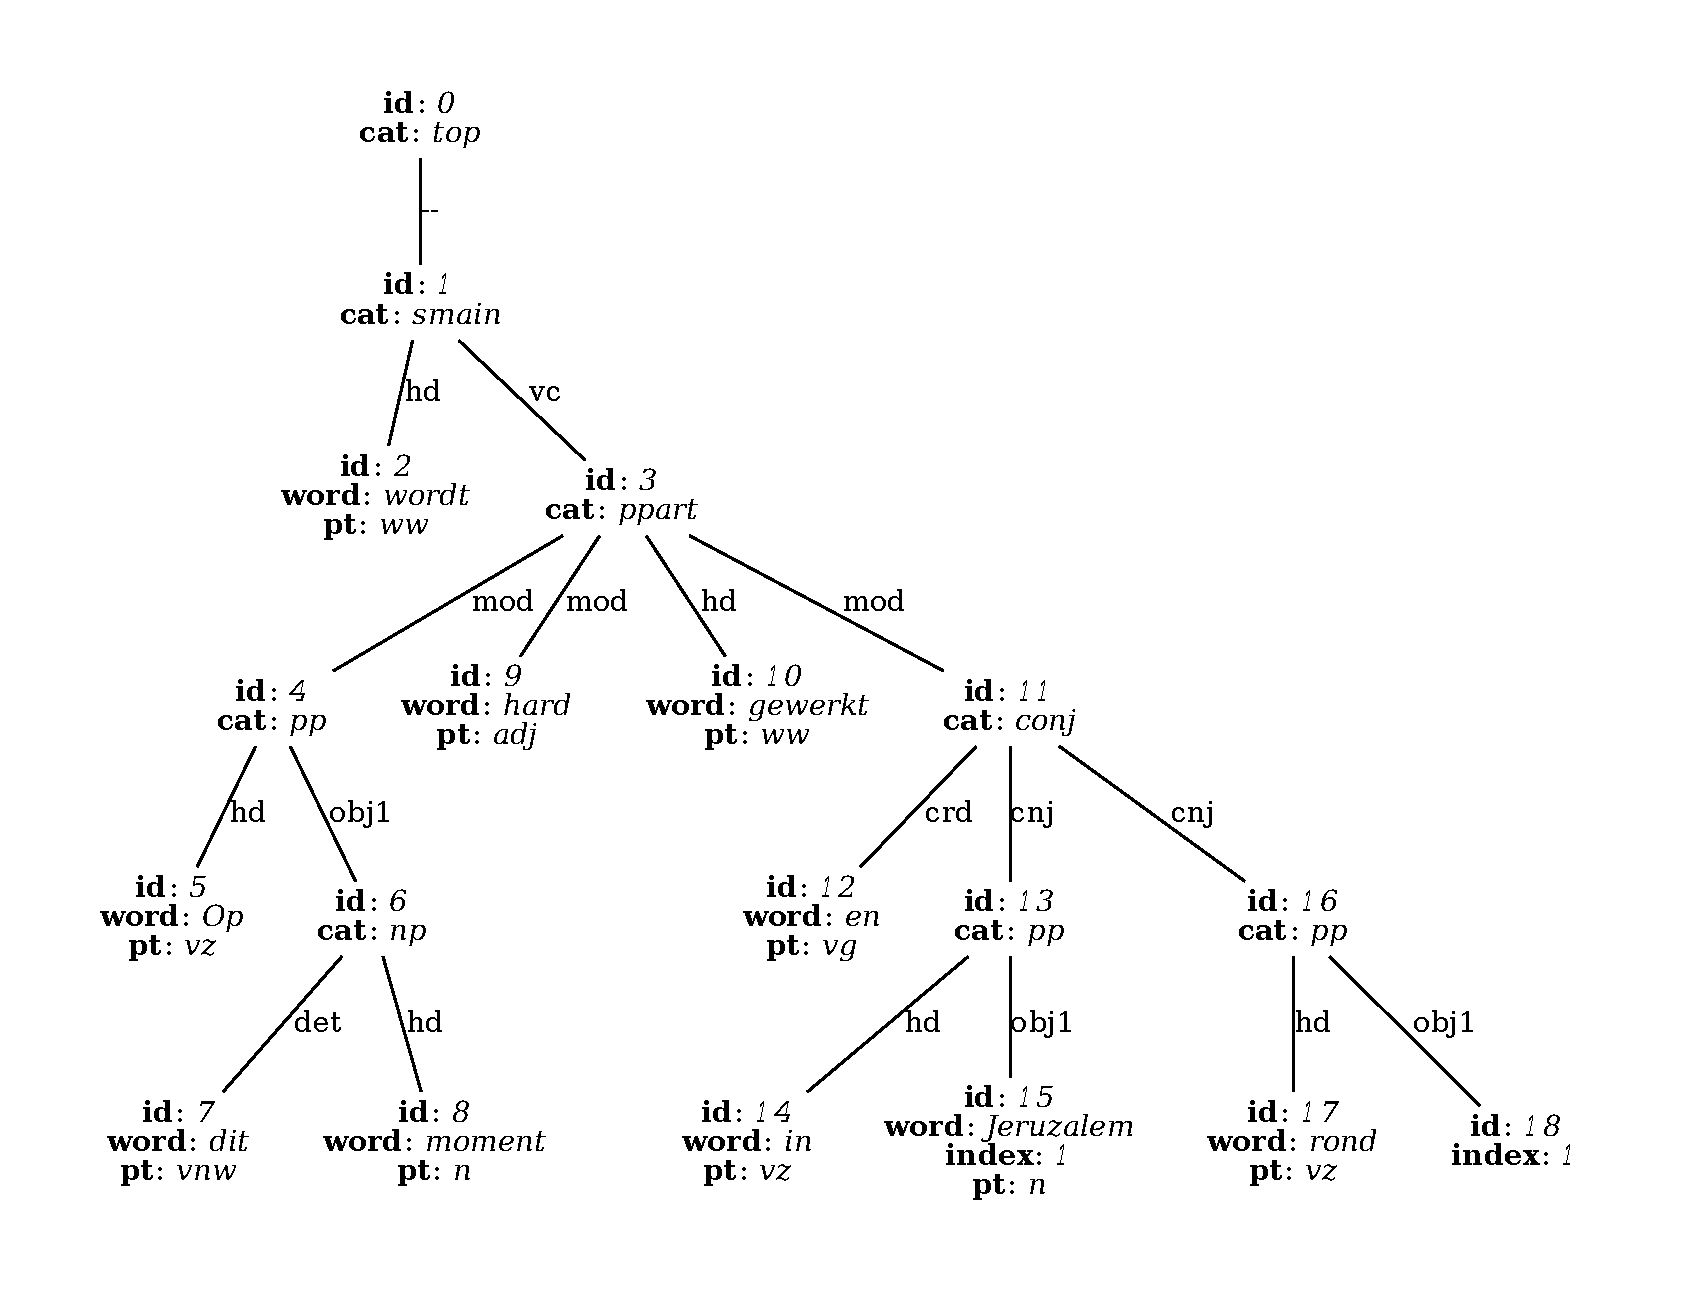
\includegraphics[width=1\textwidth]{./prebuilt/parse_example.pdf}
	\lassycap
		{WS-U-E-A-0000000013.p.37.s.1}
		{Op dit moment wordt hard gewerkt in en rond Jeruzalem.}
		{At the moment there is hard work being done in and around Jerusalem.}
	\caption{Example Lassy graph. Note the identification of nodes 15 and 18 by a common index, marking the double use of \textex{Jeruzalem} as the direct object of prepositioal phrases 13 and 16.}
	\label{figure:example_lassy_tree}
\end{figure}

\begin{table}
	\centering
	\begin{tabularx}{0.925\textwidth}{@{}cccc@{}}
	      \textbf{Tag} & \textbf{Description} & \textbf{Frequency} (\%) & \textbf{Assigned Type}\\
	      \toprule
	      \multicolumn{4}{@{}c@{}}{Lassy Short POS Tags}\\
	      \midrule[0.005pt]
	      \textit{adj} & Adjective & 7.3 & \adj[s]\\
	      \textit{bw} & Adverb & 4.5 & \bw[s]\\
	      \textit{let} & Punctuation & 11.2 & \letter[s]\\
	      \textit{lid} & Article & 10.7 & \lid[s]\\
	      \textit{n} & Noun & 22.5 & \n[s]\\
	      \textit{spec} & Special Token & 3.5 & \n[s]\\
	      \textit{tsw} & Interjection & $<$0.1 & \tsw[s]\\
	      \textit{tw} & Numeral & 2.4 & \tw[s]\\
	      \textit{vg} & Conjunction & 4.2 & \vg[s]\\
	      \textit{vnw} & Pronoun & 6.5 & \vnw[s]\\
	      \textit{vz} & Preposition & 13.7 & \vz[s]\\
	      \textit{ww} & Verb & 13.2 & \ww[s]\\
	      \midrule[0.005pt]
	      \multicolumn{4}{@{}c@{}}{Lassy Phrasal Categories}\\
	      \midrule[0.005pt]
	      \textit{advp} & Adverbial Phrase & 0.6 & \adv[s]\\
	      \textit{ahi} & Aan-Het Infinitive & $<$0.1 & \ahi[s]\\
	      \textit{ap} & Adjectival Phrase & 2.1 & \adjp[s]\\
	      \textit{cp} & Complementizer Phrase & 3.3 & \cp[s]\\
	      \textit{detp} & Determiner Phrase & 0.2 & \detp[s]\\
	      \textit{inf} & Bare Infinitival Phrase & 4.7 & \infp[s]\\
	      \textit{np} & Noun Phrase & 36.7 & \np[s]\\
	      \textit{oti} & Om-Te Infinitive & 0.8 & \oti[s]\\
	      \textit{pp} & Prepositional Phrase & 23.2 & \pp[s]\\
	      \textit{ppart} & Past Participial Phrase & 4.2 & \ppart[s]\\
	      \text{ppres} & Present Participial Phrase & 0.1 & \ppres[s]\\
	      \textit{rel} & Relative Clause & 1.9 & \rel[s]\\
	      \textit{smain} & SVO Clause & 4.7 & \smain[s]\\
	      \textit{ssub} & SOV Clause & 0.8 & \ssub[s]\\
	      \textit{sv1} & VSO Clause & $<$0.1& \svi[s]\\
	      \textit{svan} & Van Clause & $<$0.1 & \svan[s]\\
	      \textit{ti} & Te Infinitive & 1.8 & \ti[s]\\
	      \textit{whq} & Main WH-Q & 0.1 & \whq[s]\\
	      \textit{whrel} & Free Relative & 0.2 & \whrel[s]\\
	      \textit{whsub} & Subordinate WH-Q & 0.2 & \whsub[s]\\
	      \textit{du} & Discourse Unit & 2.6 & --\\
	      \textit{mwu} & Multi-Word Unit & 5.9 & --\\
	      \textit{conj} & Conjunct & 5.7 & --
	\end{tabularx}
	\caption{Lassy POS tags and phrasal category labels, and corresponding atomic types.}
	\label{table:catset}
\end{table}

\begin{table}
	\centering
	\begin{tabularx}{0.925\textwidth}{@{}cccc@{}}
	      \textbf{Label} & \textbf{Description} & \textbf{Frequency} (\%) & \textbf{Modality}\\
	      \toprule
	      \textit{app} & Apposition & 0.8 & $\dbox{app}$\\
	      \textit{body} & WH-question Body & 0.1 & $\ddia{whbody}$\\
	      \textit{body} & Relative Clause Body &0.1& $\ddia{relcl}$\\
	      \textit{body} & Complementizer body & 2 & $\ddia{cmpbody}$\\
	      \textit{cnj} & Conjunct &4.3& $\ddia{cnj}$\\
	      \textit{crd} & Coordinator &1.9& --\\
	      \textit{det} & Determiner &9.7& $\dbox{det}$\\
	      \textit{dlink} & Discourse Link & 0.2 & --\\
	      \textit{dp} & Discourse Part & 0.8 & --\\
	      \textit{hd} & Phrasal Head & 27.8 &-- \\
	      \textit{hdf} & Final Part of Circumposition & $<$0.1 & $\ddia{hdf}$\\
	      \textit{ld} & Locative Complement &0.5& $\ddia{ld}$\\
	      \textit{me} & Measure Complement &0.1& $\ddia{me}$\\
	      \textit{mod} & Modifier &16.4& $\dbox{mod}$\\
	      \textit{mwu} & Multi-word Part &5.1& --\\
	      \textit{nucl} & Nuclear Clause &0.5& --\\
	      \textit{obcomp} & Comparison Complement &0.1& $\ddia{obcomp}$\\      
	      \textit{obj1} & Direct Object &10.8& $\ddia{obj1}$\\
	      \textit{obj2} & Secondary Object &0.2& $\ddia{obj2}$\\
	      \textit{pc} & Prepositional Complement &10.6& $\ddia{pc}$\\      
	      \textit{pobj1} & Preliminary Direct Object &$<$0.1& $\ddia{pobj1}$\\      
	      \textit{predc} & Predicative Complement &1.3& $\ddia{predc}$\\      
	      \textit{predm} & Predicative Modifier &0.1& $\dbox{predm}$\\      
	      \textit{sat} & Satellite &0.2& --\\
	      \textit{se} & Obligatory Reflexive Object &0.7& $\ddia{se}$\\      
	      \textit{su} & Subject &6.9& $\ddia{su}$\\
	      \textit{sup} & Preliminary Subject &$<$0.1& $\ddia{sup}$\\
	      \textit{svp} & Separable Verbal Participle &0.7& $\ddia{svp}$\\   
	      \textit{vc} & Verbal Complement &2.8& $\ddia{vc}$\\
	      \textit{tag} & Appendix &0.1& $\ddia{tag}$\\
	      \textit{whd} & WH-question Head &0.1 & --\\
	      \textit{rhd} & Relative Clause Head & 0.1 & --\\
	\end{tabularx}
	\caption{Lassy dependency labels, and corresponding modalities.}
	\label{table:depset}
\end{table}


\section{Extraction Algorithm}
The stage is set.
We need to devise an algorithm that accepts trees like the one of Figure~\ref{figure:example_lassy_tree} and spits out proofs in $\NLP_{\diamond,\bx}$.
For such an endeavour to be successful, we must first do our best to ensure that the tree is in fact compatible with the target logic, which is unfortunately not always the case.
The first step is therefore to massage any rough edges with a series of transformations aimed at fixing inconsistent formattings and underspecified annotations.

\subsection{Transformations}
Despite its admittedly high quality, Lassy has not been built with a strong focus towards compositionality.
This reflects in several design decisions that de facto necessitate some global concessions and adaptations, and some local emergency measures, ranging from targeted transformations in the best case, to occassionally just giving up on a sample in the worst.

\subsubsection{Non-Compositional Annotations}
The biggest problem that we are faced with right off the boat is the abundance of generic, multi-purpose annotation schemes to convey non-compositional or underanalyzed syntactic structures.
These come in two flavours -- discourse level annotations, and multi-word phrases.

\paragraph{Discourse Level Annotations}
Discourse level annotations are materialized by dependencies \textit{dlink}, \textit{dpart}, \textit{nucl} and \textit{sat}, used in a catch-all fashion in place of an actual syntactic analysis.
In the example of Figure~\ref{figure:du_mwp_example} the two sentences are analyzed as ``discourse parts'' of a single ``discourse unit'' rather than matrix clauses joined by the comma -- with some goodwill we could let that slide, but that same strategy is internally applied within the second sentence (apparently a ``discourse unit'' rather than a sentence), thus avoiding a proper justification for the elided verb. 
Unfortunatey, there is no algorithmic way to mend these pretend annotations, in part due to their wildly general use, but mostly due to the fact they give us nothing to work with.
This phenomenon is unpleasantly common; discourse level annotations sum up to about 2\% of the total dependency edges in the corpus, and are present in some 11\,700 samples, polluting a hard to ignore 18\% of the dataset.
In order not to lose all the precious samples in their totality, rather than discard the entire tree we take the more conservative approach of simply pruning the problematic edges.
The subtree underneath each cut is subsequently rooted independently, sprouting an array of smaller samples from the original
%. and rooting the trees remaining underneath as independent samples.

%\begin{figure}
%	\begin{tikzpicture}
%	\begin{semilogxaxis}[
%	    title={Type Assignments/Occurrence Counts},
%	    xlabel={Occurrence Count},
%	    ylabel={Proportion of Type Assignments},
%	    xmin=1, xmax=140000,
%	    ymin=-0, ymax=1,
%	    xtick={1,10,100,1000,10000, 100000},
%	    legend pos=north west,
%	    ymajorgrids=true,
%		minor y tick num=1,
%	    yminorgrids=true,
%	    xmajorgrids=true,
%	    xminorgrids=true,
%	    axis line style={draw=none},
%	    tick style={draw=none}
%	]
%	
%	% types
%	\addplot[black, const plot, dashdotdotted, thick]
%		table[
%	    mark=none,
%	    x index=0,
%	    y index=1,
%	    col sep=comma,
%	    ] {data/proportion_of_types_covered.dat};
%	
%	% assignments
%	\addplot[black, const plot, dashed, thick]
%		table[
%	    mark=none,
%	    x index=0,
%	    y index=1,
%	    col sep=comma,
%	    ] {data/proportion_of_assignments_covered.dat};
%	
%	% sentences
%	\addplot[black, const plot]
%		table[
%	    mark=none,
%	    x index=0,
%	    y index=1,
%	    col sep=comma,
%	    ] {data/proportion_of_sentences_covered.dat};
%	    
%	\end{semilogxaxis}
%	\end{tikzpicture}
%	\label{figure:plot:assignment_occurrence_ecdf}
%\end{figure}



\bibliographystyle{abbrvnat}
\bibliography{bibliography}